
\documentclass[a4paper,10pt]{report}
\usepackage{blindtext} % for dummy texts
\usepackage[T1]{fontenc}
\usepackage[table]{xcolor}
\usepackage{titlesec}
\usepackage{graphicx}
\usepackage[inkscapepath=../assets/svg]{svg}
\usepackage{amsmath}
\usepackage{amsthm}
\usepackage{float}
\usepackage{mathtools}
\usepackage{fancyvrb}
\usepackage[english]{babel}
\usepackage{csquotes}
\usepackage{hyperref}
\hypersetup{
   colorlinks=true,
   linkcolor=blue,
   urlcolor=cyan
}
\usepackage{tikz}
\usepackage{amssymb}
\usepackage[sc]{mathpazo}
\linespread{1.05}
\usepackage{microtype}
\usepackage{breqn}
\usepackage{caption}
\usepackage{subcaption}
\usepackage[
   backend=bibtex,%
   bibencoding=utf8,%
   language=english,%
   style=numeric-comp,%
   sorting=nyt,%
   maxbibnames=10,%
   natbib=true%
]{biblatex}
\addbibresource{references.bib}
\usepackage{siunitx}
\usepackage{booktabs}
\usepackage{longtable}
\usepackage{geometry}
\usepackage{multirow}
\graphicspath{ {../assets/img/} }

\newgeometry{hmargin={30mm,30mm}}

% Set TOC depth and sections numbering
\setcounter{tocdepth}{3}
\setcounter{secnumdepth}{3}

% Remove chapters head and reduce spacing
\titleformat{\chapter}[hang]{\Large\bfseries}{\thechapter \hspace{2ex}}{0pt}{\Large}
\titlespacing{\chapter}{0cm}{0cm}{0.5cm}
\usepackage[parfill]{parskip}

% Make quotes italic
\renewcommand{\mkbegdispquote}[2]{\itshape}

% Change text line breaks
\renewcommand{\texttt}[1]{%
  \begingroup
  \ttfamily
  \begingroup\lccode`~=`.\lowercase{\endgroup\def~}{.\discretionary{}{}{}}%
  \catcode`/=\active\catcode`[=\active\catcode`.=\active
  \scantokens{#1\noexpand}%
  \endgroup
}

\def\lc{\left\lceil}   
\def\rc{\right\rceil}
\def\lf{\left\lfloor}   
\def\rf{\right\rfloor}


\begin{document}
\frenchspacing


%----------------------------------------------------------------------------------------
%	TITLE SECTION
%----------------------------------------------------------------------------------------
\title{
  {{\large{\textsc{Alma Mater Studiorum $\cdot$ University of Bologna}}}}
  \rule{\textwidth}{0.4pt}\vspace{3mm}
  \textbf{Machine Learning Project Report: 
Restaurant Revenue Prediction}
  \begin{figure}[!htb]
    \centering
    
\includegraphics[width = 150pt]{img/AlmaMaterLogo.png}
  \end{figure} \\
   Machine Learning
}

\author{ Tiberio Marras (\href{mailto:tiberio.marras@studio.unibo.it}{tiberio.marras@studio.unibo.it})}
\date{\today}
\maketitle
\newpage
\tableofcontents
\setcounter{tocdepth}{1}
%\listoffigures
%\listoftables
\newpage
\maketitle
\chapter{Introduction}
\section{Task description}
The task of the project is to create a reliable mathematical model able to predict the revenue of 100.000 restaurants.\\
The model is trained using the \emph{location}, the \emph{age}, the \emph{kind of city} where is located, the \emph{type} of restaurant and three categories of obfuscated data (\emph{demographic} data, \emph{real estate} data and \emph{commercial} data).\\
The model to find is a \emph{regressor} which, given the features, must predict the eventual revenue of the restaurant.\\
The target doesn't strictly represent the real revenue but a number which relates to it.\\
The metric used to compare the results is \emph{Root Mean Squared Error} (RMSE) over the 100.000 predictions.
$$
RMSE = \sqrt{\frac{1}{n}\sum_{i=1}^{n}(y_{i} - \hat{y_{i}})^2}
$$
\section{Background}
The regression is an approach for modelling the relationship between a scalar response and one or more explanatory variables.\\
The case of one explanatory variable is called \emph{simple regression}; for more than one, the process is called \emph{multiple regression}.\\
The relationships  between the dipendent and the indipendent variables are modeled using predictor functions whose unknown model parameters are estimated from the data.\\
In machine learning there are several kinds of regressors such as \emph{linear regressor}, \emph{Ridge regressor}, \emph{Lasso regressor} and others which we will see in the following sections.\\
Solving regression problems is one of the most common applications for machine learning models, especially in \emph{supervised machine learning}. Algorithms are trained to understand the relationship between independent variables and an outcome or dependent variable. The model can then be leveraged to predict the outcome of new and unseen input data, or to fill a gap in missing data.\\
Common use for machine learning regression models include: 
 
\begin{itemize}
\item Forecasting continuous outcomes like house prices, stock prices, or sales.
\item Predicting the success of future retail sales or marketing campaigns to ensure resources are used effectively. 
\item Predicting customer or user trends, such as on streaming services or ecommerce websites. 
\item Analysing datasets to establish the relationships between variables and an output. 
\item Predicting interest rates or stock prices from a variety of factors. 
\item Creating time series visualisations. 
\end{itemize}

Some of the most common regression techniques in machine learning can be grouped into the following types of regression analysis: 
\begin{itemize}
\item Simple Linear Regression 
\item Multiple linear regression 
\item Logistic regression 
\end{itemize}
To follow a graph representing the \emph{Simple Linear Regression}.
\\
\\
\\
\begin{figure}[H]
    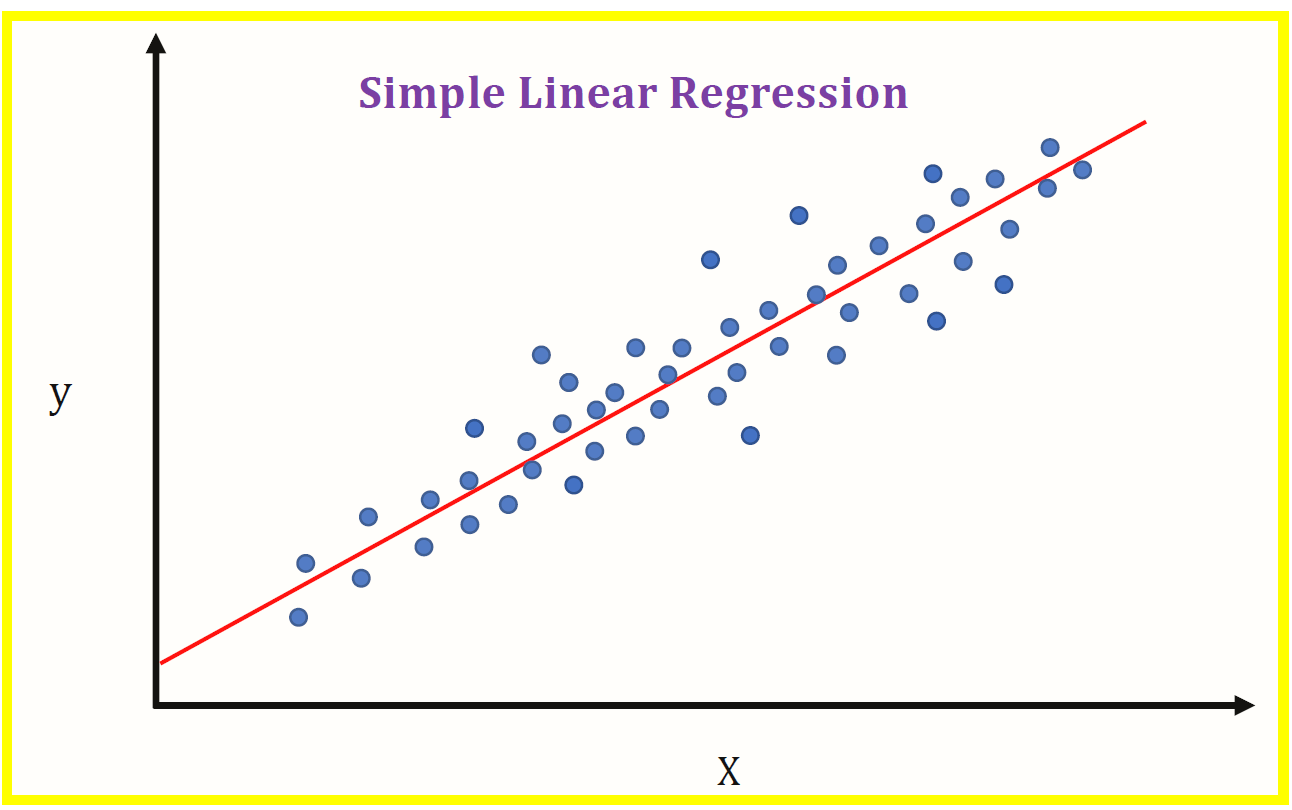
\includegraphics[width = 400pt]{img/simplelinregr.png}
  \end{figure} 
\chapter{The dataset}
The dataset for the training is composed of 137 records representing restaurants.\\
Each row has 42 columns for the features and 1 column for the target.\\
The test set is composed of 100.000 records representing restaurant for which to predict the revenue. The test set doesn't contain the target variable.\\
\section{Composition}
The features for the training are:
\begin{itemize}
\item \emph{Id} - the id of the row
\item \emph{Open date} - opening date for a restaurant
\item \emph{City} - the city of the restaurant
\item \emph{City group} - the type of city. Big cities or others.
\item \emph{Type} - type of the restaurant. FC: Food Court, IL: Inline, DT: Drive Thru, MB: Mobile
\item \emph{P1, P2 - P37} - obfuscated data representing three categories:  Demographic data are gathered from third party providers with GIS systems. These include population in any given area, age and gender distribution, development scales. Real estate data mainly relate to the m2 of the location, front facade of the location, car park availability. Commercial data mainly include the existence of points of interest including schools, banks, other QSR operators.
\end{itemize}
The target is the transformed revenue, since it is transformed it doesn't represent real dollar value.
\section{Inspect the dataset}
First I inspect the revenue.
\begin{figure}[H]
    \centering
    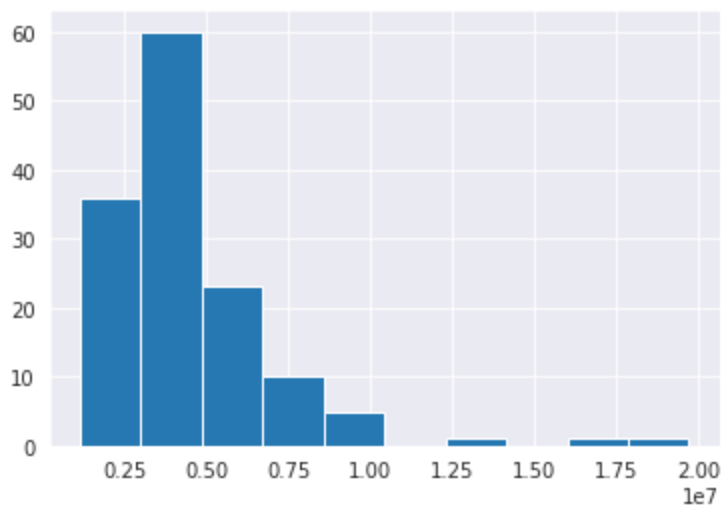
\includegraphics[width = 300pt]{img/revenue.png}
  \end{figure} 
We can say that the majority of restaurants has \emph{low} revenue. This can be caused by many factors.\\
I also created a new feature which computes the number of days since the opening date in order to evaluate the age of the restaurant.\\
\begin{figure}[H]
    \centering
    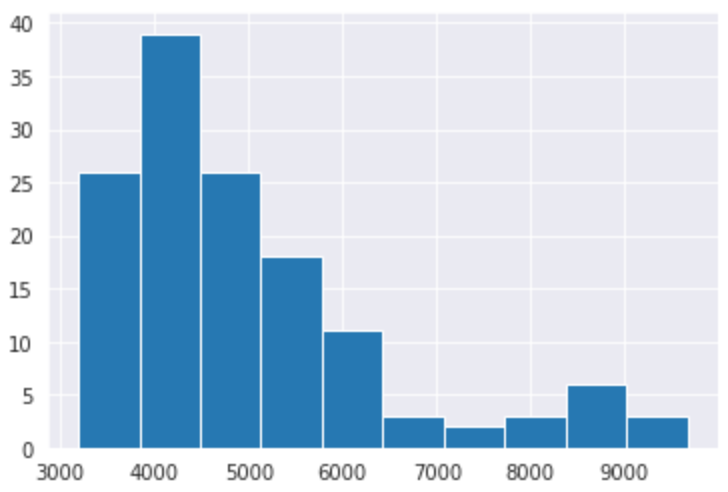
\includegraphics[width = 300pt]{img/opendate.png}
  \end{figure} 
We can say that the majority of restaurants has a \emph{young} age. This is because statistically it is more likely for a restaurant to fail after a certain amount of time.
\begin{figure}[H]
    \centering
    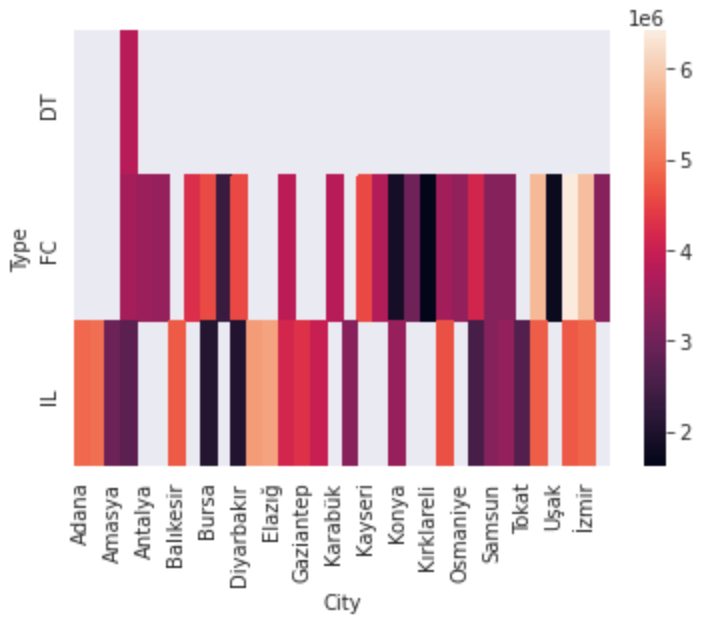
\includegraphics[width = 300pt]{img/revenuepivot.png}
  \end{figure} 
In this map the color of the cells is the revenue, we can also say that DT restaurants are not good at all.
\begin{figure}[H]
    \centering
    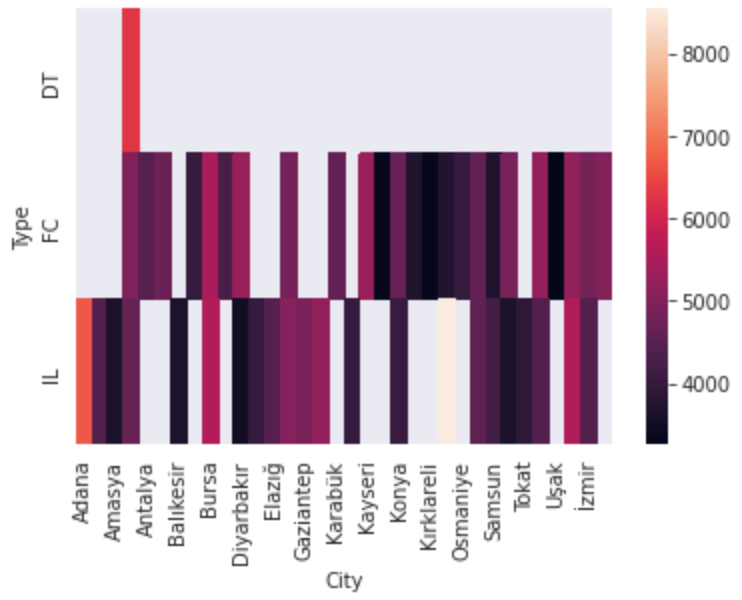
\includegraphics[width = 300pt]{img/opendatepivot.png}
  \end{figure} 
In this map the color of the cells is the open date. As we already said the majority of restaurants has a young age, and this doesn't make much difference between IL and FC restaurants.
\begin{figure}[H]
    \centering
    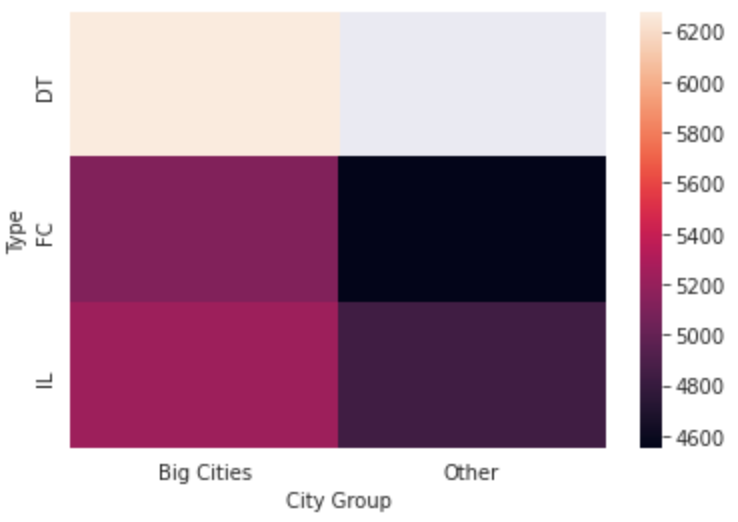
\includegraphics[width = 300pt]{img/citygrouppivot.png}
  \end{figure} 
In this map the color of the cells is the open date. As we can see restaurants in big cities tend to last more than restaurants in other cities, this is probably for the bigger number of customers which is easier to reach in big cities.
\begin{figure}[H]
    \centering
    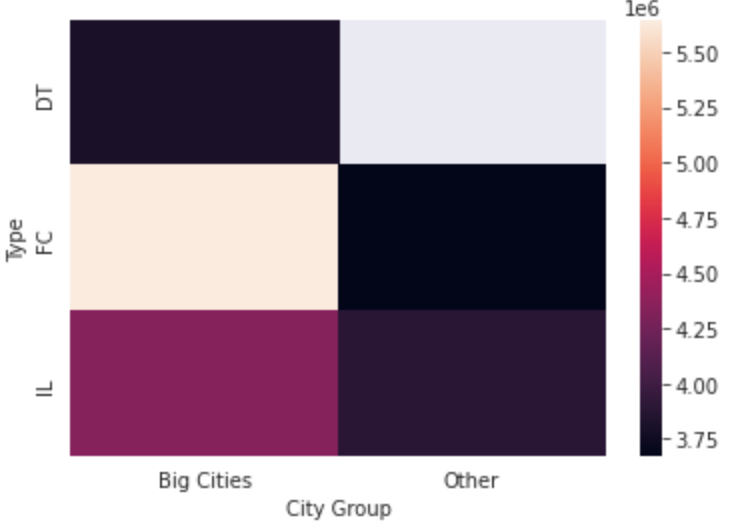
\includegraphics[width = 300pt]{img/revenuecitygrouppivot.png}
  \end{figure}
  In this map the color of the cells is the revenue. We can say that FC and IL restaurants tend to have bigger revenues in big cities than in other cities.
\section{Preprocessing}
I performed two different preprocessings for the classic regressors and the neural network.\\
\subsection{Classic regressors}
For the classic regressors I used {\fontfamily{cmtt}\selectfont
SimpleImputer} to fill the missing values in the dataset using the \emph{median} as descriptive statistic.\\
Then I standardized numerical values using the {\fontfamily{cmtt}\selectfont StandardScaler}.\\
I decided to perform standardization in order to make the models converge faster and reduce the computation time of training.\\
For the \emph{city group} I used the {\fontfamily{cmtt}\selectfont OrdinalEncoder} which encodes the categorical values as integers.\\
In this case I decided to use {\fontfamily{cmtt}\selectfont OrdinalEncoder} because of the fact that the categories are only two.
For the \emph{type} of restaurant I used {\fontfamily{cmtt}\selectfont OneHotEncoder} which encodes the categorical values ad one-hot encoded arrays.\\
In this case, differently from the \emph{city group}, the number of categories is greater than 2, this is why I decided to perform one-hot encoding.\\
In order to reduce the number of features I used \emph{PCA} with a number of components equal to 0.99.
This way the number of features became 27.
\subsection{Neural network}
For the neural network I performed the same preprocessing steps except for the {\fontfamily{cmtt}\selectfont StandardScaler} for the numerical features.\\
In this case I used a {\fontfamily{cmtt}\selectfont MinMaxScaler} instead, which scales the feature using the min - max range.\\
I decided not to use standardization in this case in order not to change the distribution of data.\\
I used \emph{PCA} to reduce the number of features with the neural network as well, but this time with number of components equal to 0.95.\\
This way I reduced the number of features to 13.
\chapter{Methods}
To find the best regression model I performed a {\fontfamily{cmtt}\selectfont GridSearchCV} over various regressors (included the neural network) and I compared the results.\\
For the classic regressors I tried with various combinations of parameters the following ones:
\begin{itemize}
\item \emph{Support Vector Regressor} (I tuned on Kernel, Epsilon, Gamma and C)
\item \emph{AdaBoost Regressor} (I tuned on n\_estimators, learning\_rate and random\_state)
\item \emph{KNeighbors Regressor} (I tuned on n\_neightbors, weights and metric)
\item \emph{SGD Regressor} (I tuned on Alpha, max\_iter, loss and Penalty)
\item \emph{Ridge} (I tuned on Alpha)
\item \emph{Lasso} (I tuned on Alpha)
\end{itemize}
During the loop on {\fontfamily{cmtt}\selectfont GridSearchCV} I create 2 dictionaries with the best parameters and the best score for each regressor.\\
Using these dictionaries the program can compare each result in order to find the best regressor available.\\
In the case of the neural network I created a function {\fontfamily{cmtt}\selectfont create\_model()} which takes various parameters for the creation of the model.\\
The parameters I tuned on are \emph{Batch\_size}, \emph{Epochs}, \emph{Learning\_rate}, \emph{Momentum}, \emph{Dropout\_rate}.
I tried various architectures changing the number of layers, the number of hidden nodes and the activation functions.\\
The activation function is the classic \emph{Relu} for the hidden layers and \emph{Sigmoid} for the output layer.\\
After tuning on the neural network I compared the result of {\fontfamily{cmtt}\selectfont GridSearchCV} on the neural network with the one of the best regressor found.\\
For the cross-validation of {\fontfamily{cmtt}\selectfont GridSearchCV} I used 5 folds and I used \emph{Negative Root Mean Square Error} as scoring to compare the results.


\chapter{The environment}
The environment I used is a \emph{Python 3} notebook with \emph{Colab}.
I created a directory in my \emph{Google Drive} with the project and a subdirectory with the dataset.
I used the \emph{Drive} library of \emph{Colab} to mount the path to the directory in order to fetch the training and the test datasets to load on a dataframe.\\
The output file with the results on the test set is located on the same subdirectory of the dataset.\\
I used the free version of \emph{Colab} with standard \emph{RAM} and \emph{Disk}.\\
The \emph{Colab} environment has 2 processors \emph{Intel(R) Xeon(R)} with 1 core each.\\
Each processor has a \emph{frequency clock} of 2200.218 MHz and a \emph{cache size} of 56320 Kb.\\
To follow the charasteristics of one processor on \emph{Colab}.
\begin{figure}[H]
    \centering
    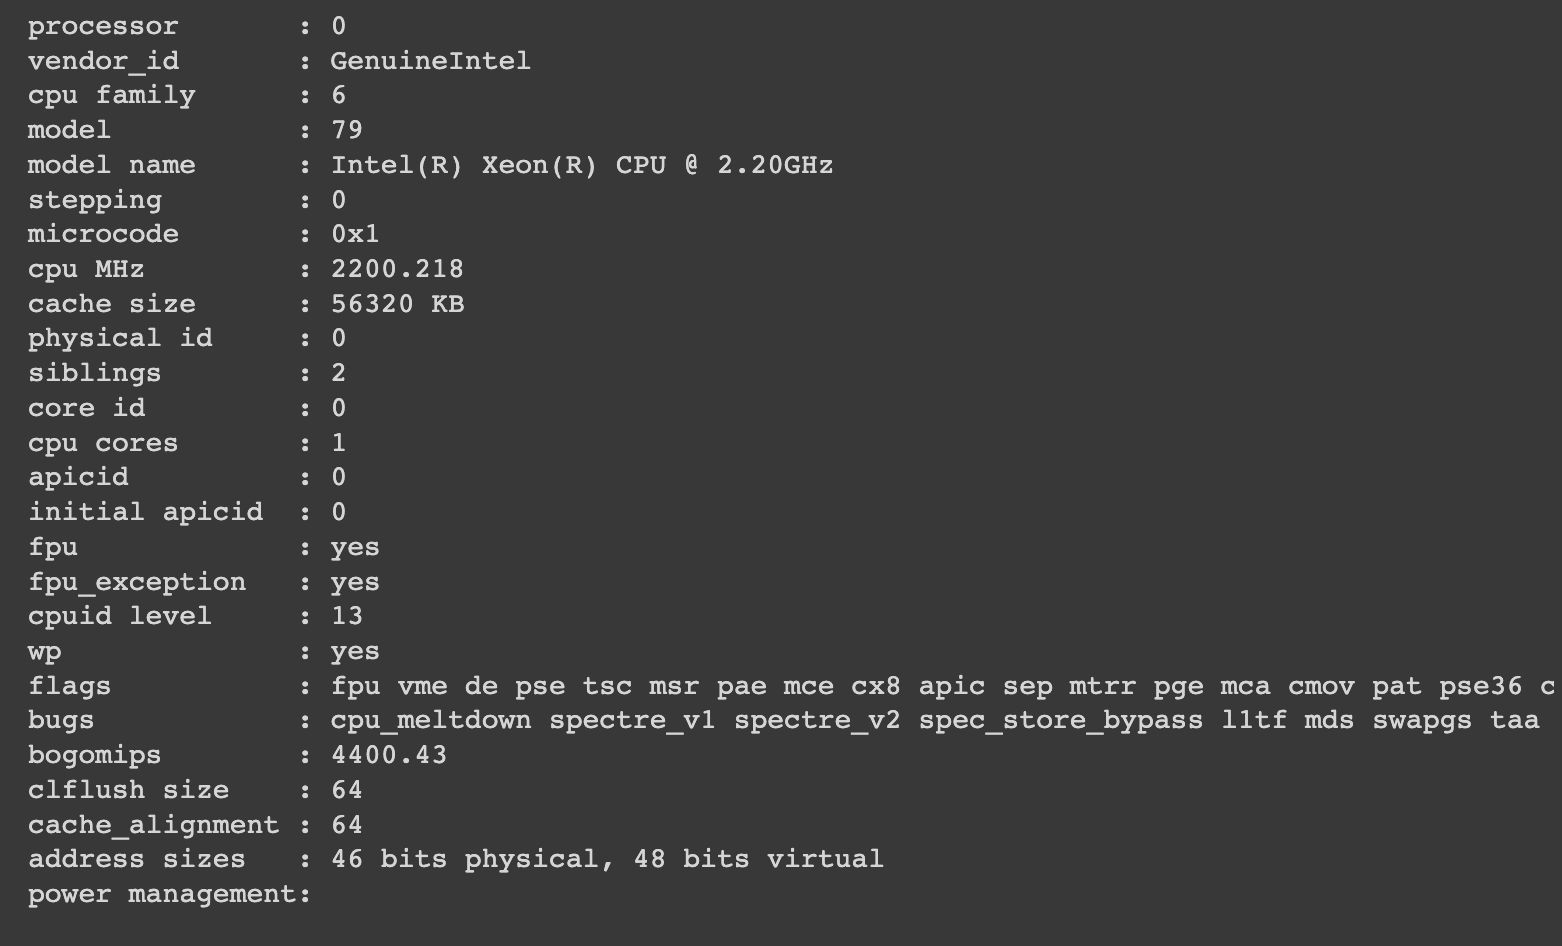
\includegraphics[width = 400pt]{img/procchar.png}
  \end{figure}
As a first step I had to perform {\fontfamily{cmtt}\selectfont !pip install scikeras} since the library wasn't available by default on \emph{Colab.}
\chapter{Results}
The best model resulted to be \emph{KNeighbors Regressor} with a \emph{Negative Mean Squared Error} of -5795686580515.175.
I obtained this result with the following combination of parameters:
\begin{itemize}
\item \emph{Metric}: "Manhattan"
\item \emph{N\_neightbors}: 15
\item \emph{Weigths}: "Distance"
\end{itemize}

To follow the result score for each regressor (with GridSearchCV).
\begin{figure}[H]
    \centering
    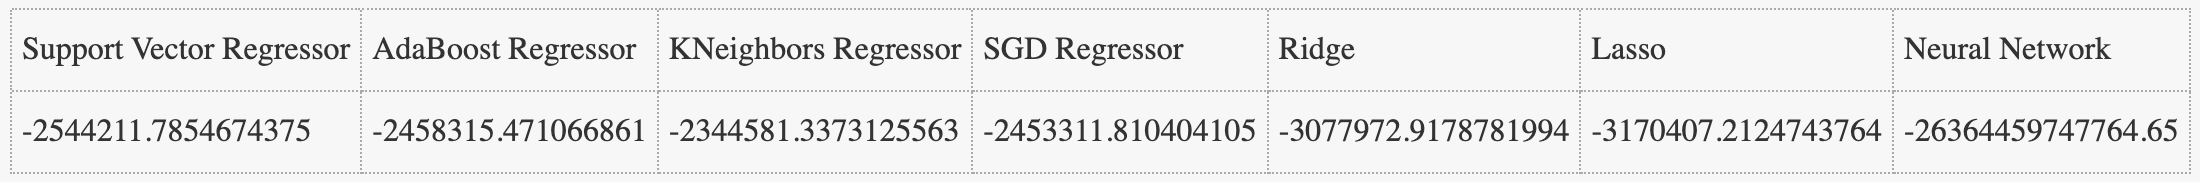
\includegraphics[width = 500pt]{img/table.png}
  \end{figure}
To follow the best parameters for each regressor.
\begin{figure}[H]
    \centering
    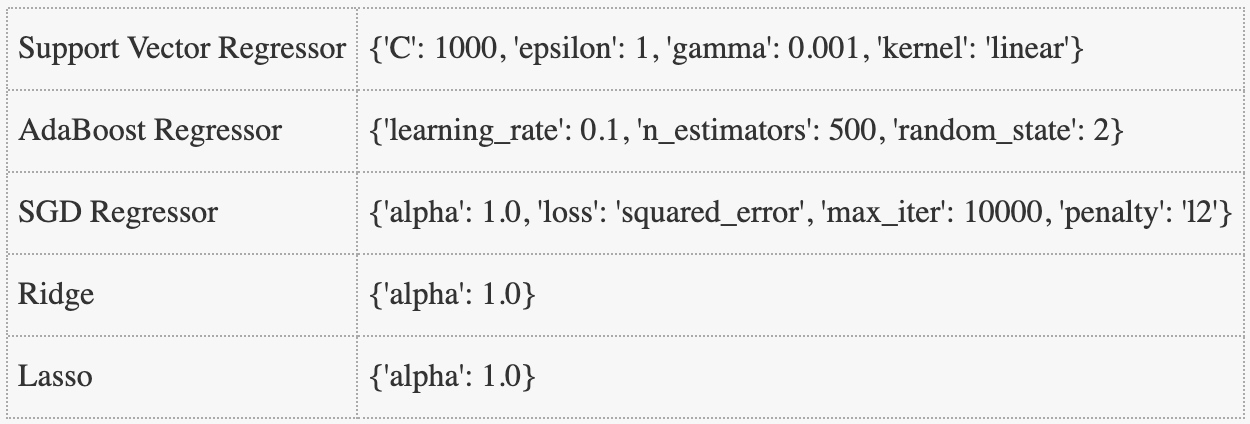
\includegraphics[width = 500pt]{img/regrparams.png}
  \end{figure}

For the neural network I obtained the best result with the following combination of parameters:
\begin{itemize}
    \item \emph{Batch\_size}: 8
    \item \emph{Epochs}: 60
    \item \emph{Learning\_rate}: 0.01
    \item \emph{Momentum}: 0.2
    \item \emph{Dropout\_rate}: 0.2
\end{itemize}
The best architecture I found counts 4 \emph{dense layers} (plus the \emph{input layer}) with 16, 8, 4 and 1 \emph{nodes} and 3 \emph{dropout layers} with a dropout rate of 0.2.\\
To follow the architecture of the neural network.
\begin{figure}[H]
    \centering
    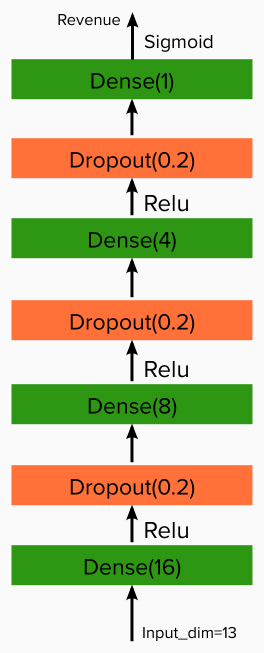
\includegraphics[height = 500pt]{img/arch.png}
  \end{figure}
\section{Conclusion}
To conclude the classic regressors seem to perform quite good compared to the \emph{neural network}, which has the 5th best result.\\
Only \emph{Ridge} and \emph{Lasso} performed worse resulting respectively in 6th and 7th position.\\
A possible explanation for this is the fact that the training set is really small compared to the test set, and since neural networks are hungry of data this could really influence the results.\\
Actually a thing to point out is that the mean \emph{Negative Root Mean Squared Error} computed on all the results is still high once all the models are trained, and this again is probably caused by the small dimension of the training set.\\
However this seems the best approach to tackle this kind of problem, also because the use of {\fontfamily{cmtt}\selectfont GridSearchCV} makes the result score more reliable. {\fontfamily{cmtt}\selectfont GridSearchCV} works even better with a bigger dataset, either with the same number of folds or increasing it.

\end{document}
